\section{Monte Carlo datasets}
For this analysis two MC productions have been used, both anchored to the 2010 pp data taking periods (LHC10b, LHC10c, LHC10d, LHC10e).
Both simulations use PYTHIA6 with the Perugia2011 tune as particle generator with $\s=7$~TeV.

The production tagged LHC14j4b, LHC14j4c, LHC14j4d, LHC14j4e is a minimum-bias production with roughly the same statistics as the one collected in real data-taking.
This production has been used to test the analysis techniques, in particular to validate the ability of the analysis chain to recover the yield of the signal.

The production tagged LHC15i2b, LHC15i2c, LHC15i2d, LHC15i2e is a production binned in $p_{\rm T,hard}$ bins.
In addition the charm content has been enhanced by requesting a \ccbar\ in 50\% of the events and a \bbbar\ in the remaining half.

Results shown below come from the LEGO train Jets\_EMC\_pp\_MC, run numbers: 949 (LHC15i2b), 950 (LHC15i2c), 951 (LHC15i2d), 952 (LHC15i2e), 953 (LHC14j4b), 954 (LHC14j4c), 955 (LHC14j4d), 956 (LHC14j4e).
\section{Overview of the analysis}
The \Dzero\ meson candidates are selected using the ``standard 2010 pp'' cuts, which are accessed through the static method AliRDHFCuts::SetStandardCutsPP2010().

For each \Dzero\ candidate a separate jet finding is performed. The daughters of the \Dzero\ candidate are 
removed from the collection of hybrid tracks; the 4-momentum of the \Dzero\ candidate is added back. 
This collection of tracks plus \Dzero\ candidate is used as input for the jet finder.
The jet finder algorithm is \antikt\ with a resolution parameter $R=0.4$ in its FastJet (v. 3.1.3) implementation.

For the estimation of the detector resolution and reconstruction efficiency, only real \Dzero\ coming from
the fragmentation of a charm quark are considered. \Dzero\ candidates are matched with generator-level \Dzero\ using their MC label.

The main analysis tasks (C++ classes) used in the analysis are in the PWGJE library:
\begin{itemize}
\item AliAnalysisTaskDmesonJets
\item AliAnalysisTaskDmesonJetsDetectorResponse
\end{itemize}
%%%%%%%%%%%%
%%%%%%%%%%%%
\section{Simulation figures}
%%%%%%%%%%%%
In the following paragraphs the figures prepared for the Hot Quarks 2016 conference are presented. Figures without the ALICE Simulation
text printed inside the canvas are not proposed as official figures to be approved.
%%%%
\subsection{Jet momentum resolution and reconstruction efficiency}
%%%%
The efficiency is taken as the ratio of the \ptd\ spectra of the D-tagged particle-level jets for which a matched
D-tagged detector-level jet was found overall the D-tagged particle-level jets (regardless of whether they are matched to a detector-level jet).
For the detector-level jets, the D meson is required to be within the standard fiducial rapidity cuts implemented in the AliRDHFCutsD0toKpi class.
Jets are further requested to have $|\eta_{\rm jet}| < 0.9 - R$, both at particle and detector levels.
Figure~\ref{fig:HQ16_Simulation_EfficiencyVsDPt} shows the jet reconstruction efficiency as a function of \ptd\ in 4 different \ptchjet\ bins.
It is noteworthy that the efficiency does not show any observable dependence on \ptchjet.
The efficiency is also shown in logarithmic scale in Fig.~\ref{fig:HQ16_Simulation_EfficiencyVsDPt_LogScale}, so as to resolve possible
differences at low momentum. From the ratios of the efficiencies in \ptchjet\ bins over the entire range, shown in Fig.~\ref{fig:D0_Jet_AKTChargedR040_pt_scheme_D_Spectra_PartialEfficiencyRatios}
one can appreciate a hint of a small deviation, on the order of 10-20\%, for low momentum \Dzero\ (\ptd~$<5$~\GeVc) in high momentum jets. However this deviation is not statistically significant.
\begin{figure}[tbh]
\begin{center}
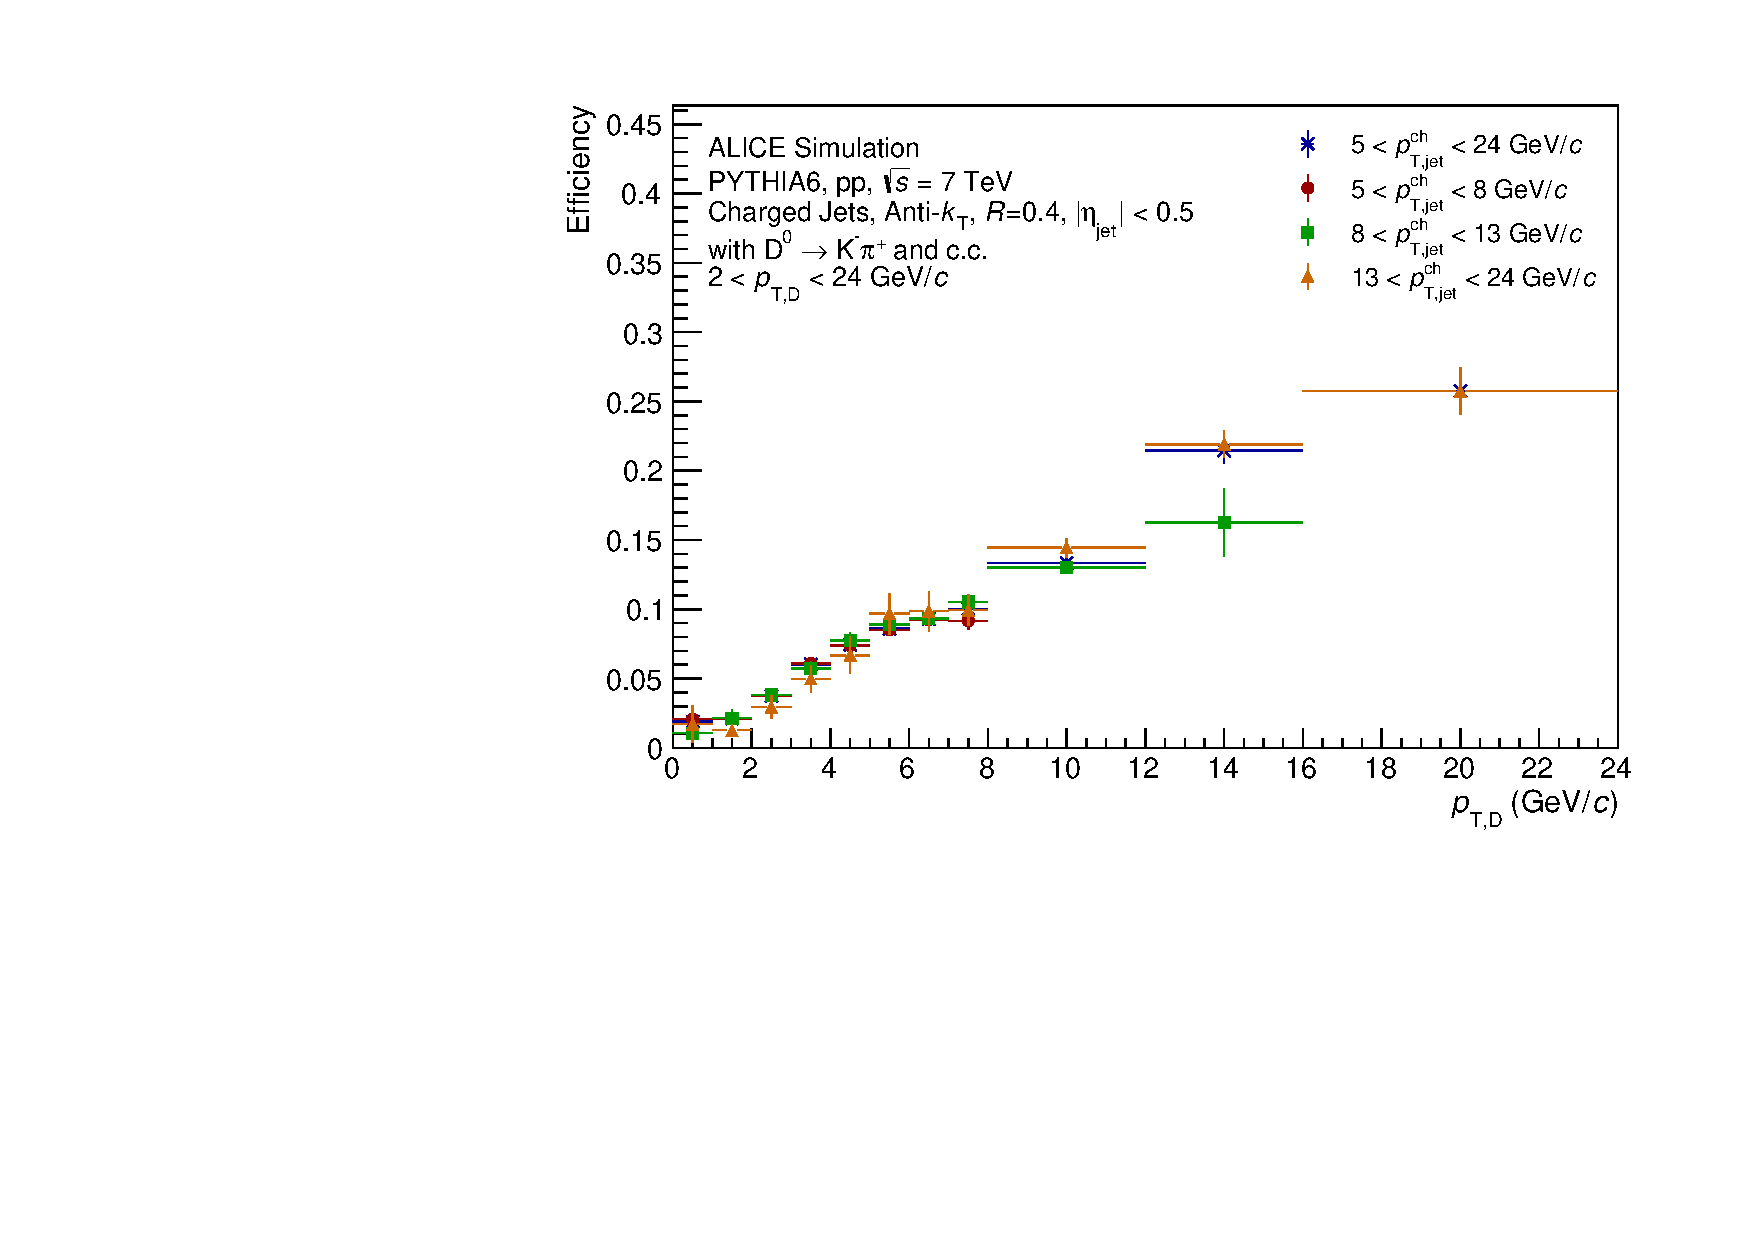
\includegraphics[width=0.8\textwidth]{img/HQ16_Simulation_EfficiencyVsDPt}
 \caption{Jet reconstruction efficiency as a function of \ptd\ in \ptchjet\ bins.} 
 \label{fig:HQ16_Simulation_EfficiencyVsDPt}
\end{center}
\end{figure}

\begin{figure}[tbh]
\begin{center}
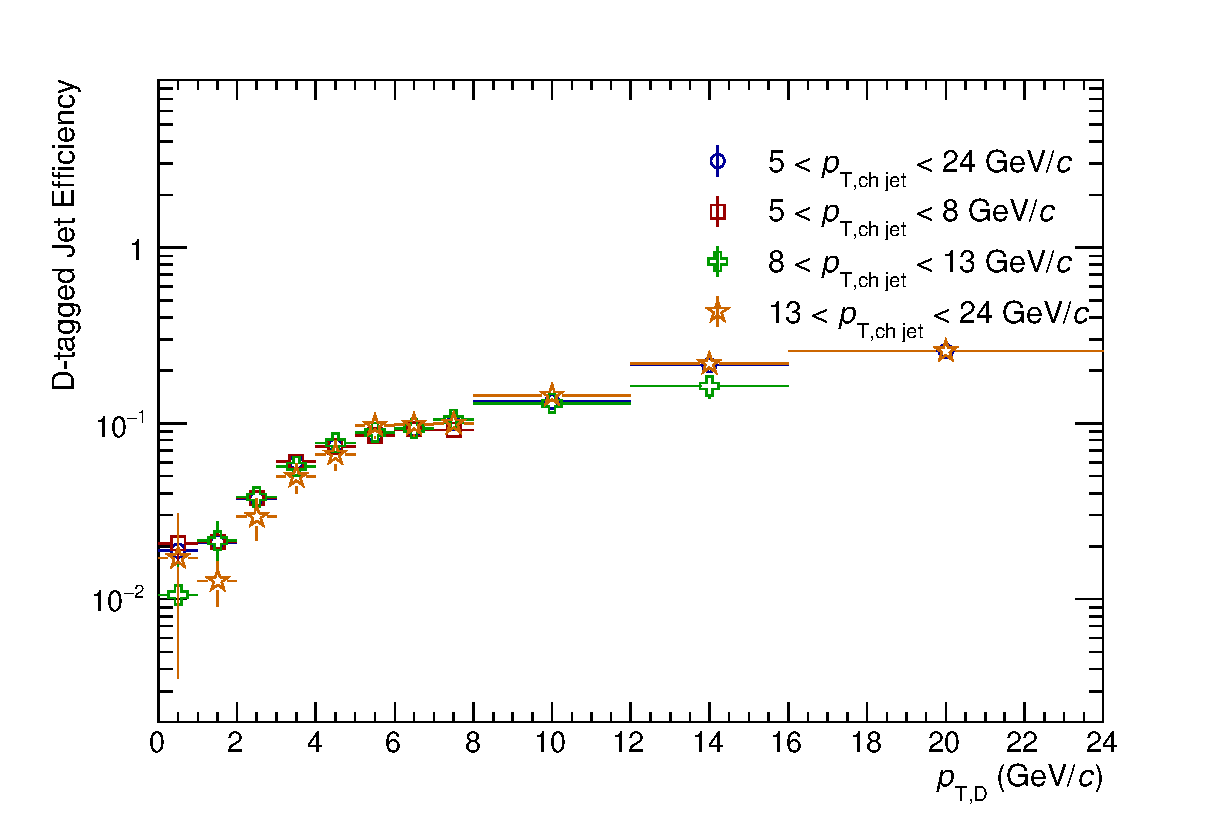
\includegraphics[width=0.8\textwidth]{img/HQ16_Simulation_EfficiencyVsDPt_LogScale}
 \caption{Jet reconstruction efficiency as a function of \ptd\ in \ptchjet\ bins.} 
 \label{fig:HQ16_Simulation_EfficiencyVsDPt_LogScale}
\end{center}
\end{figure}

\begin{figure}[tbh]
\begin{center}
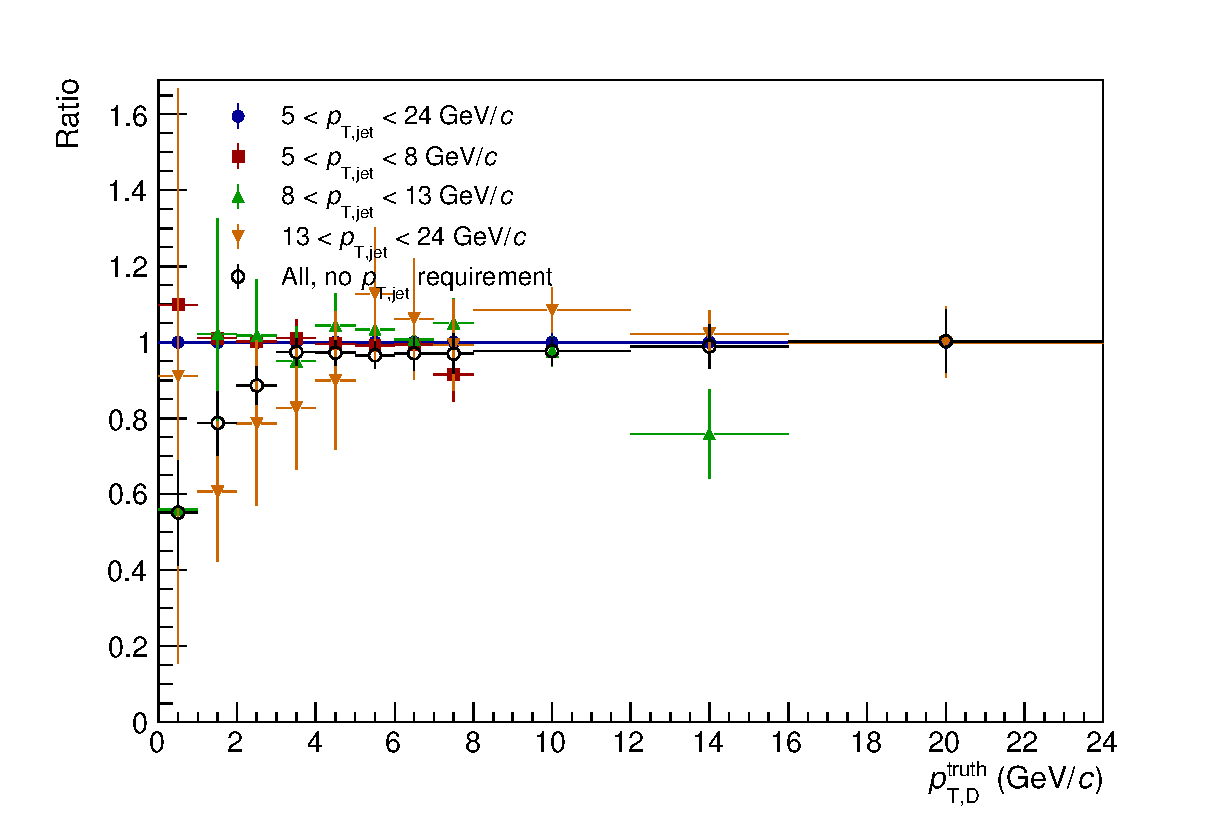
\includegraphics[width=0.8\textwidth]{img/D0_Jet_AKTChargedR040_pt_scheme_D_Spectra_PartialEfficiencyRatios}
 \caption{Ratio of the jet reconstruction efficiencies for some \ptchjet\ bins over the range $5<$~\ptchjet~$<24$~\GeVc.} 
 \label{fig:D0_Jet_AKTChargedR040_pt_scheme_D_Spectra_PartialEfficiencyRatios}
\end{center}
\end{figure}

The jet momentum resolution and energy scale shift are estimated calculating the variable:
\begin{equation}
(p_{\mathrm{T,ch\, jet}}^{\mathrm{det}} - p_{\mathrm{T,ch\, jet}}^{\mathrm{part}}) / p_{\mathrm{T,ch\, jet}}^{\mathrm{part}}
\label{eq:detResp}
\end{equation}
for each matched pair of a particle-level jet with a detector-level jet.
Figure~\ref{fig:HQ16_Simulation_DetectorResponse} shows the probability density distribution of Eq.~\ref{eq:detResp}.
The median and the mean of these distributions are shown as a function of \ptchjetgen\ in Fig.~\ref{fig:HQ16_Simulation_EnergyScaleShift}.
This gives an estimate of the relative energy scale shift that needs to be corrected for.
The jet momentum resolution is estimated looking at the standard deviation of the distribution of Eq.~\ref{eq:detResp} as a function
of \ptchjetgen, shown in Fig.~\ref{fig:HQ16_Simulation_Resolution}. The standard deviation is defined here as 
the square root of the second central moment of the distribution (also known as root-mean-square).
\begin{figure}[tbh]
\centering
\begin{subfigure}[b]{0.49\textwidth}
  \centering
  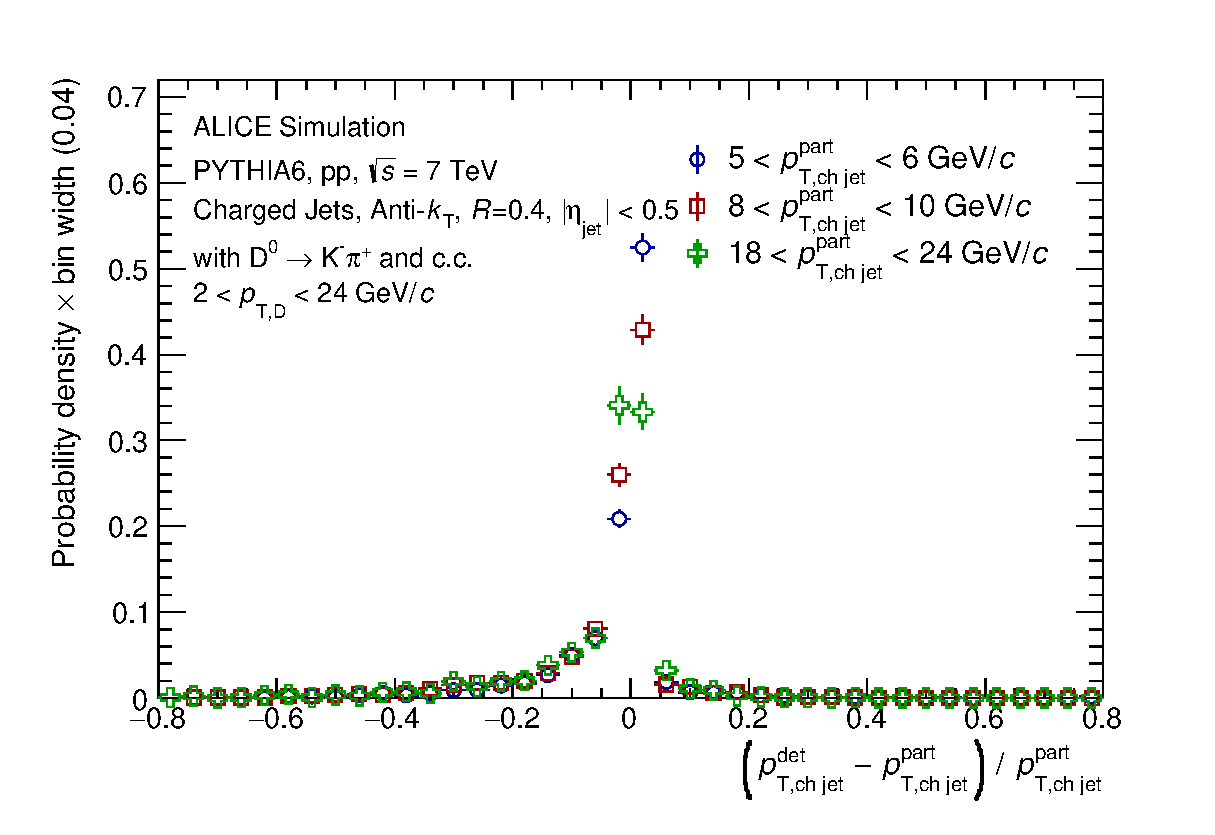
\includegraphics[width=1.0\linewidth]{img/HQ16_Simulation_DetectorResponse}
  \caption{Probability density distribution}
  \label{fig:HQ16_Simulation_DetectorResponse}
\end{subfigure}\\
\begin{subfigure}{0.49\textwidth}
  \centering
  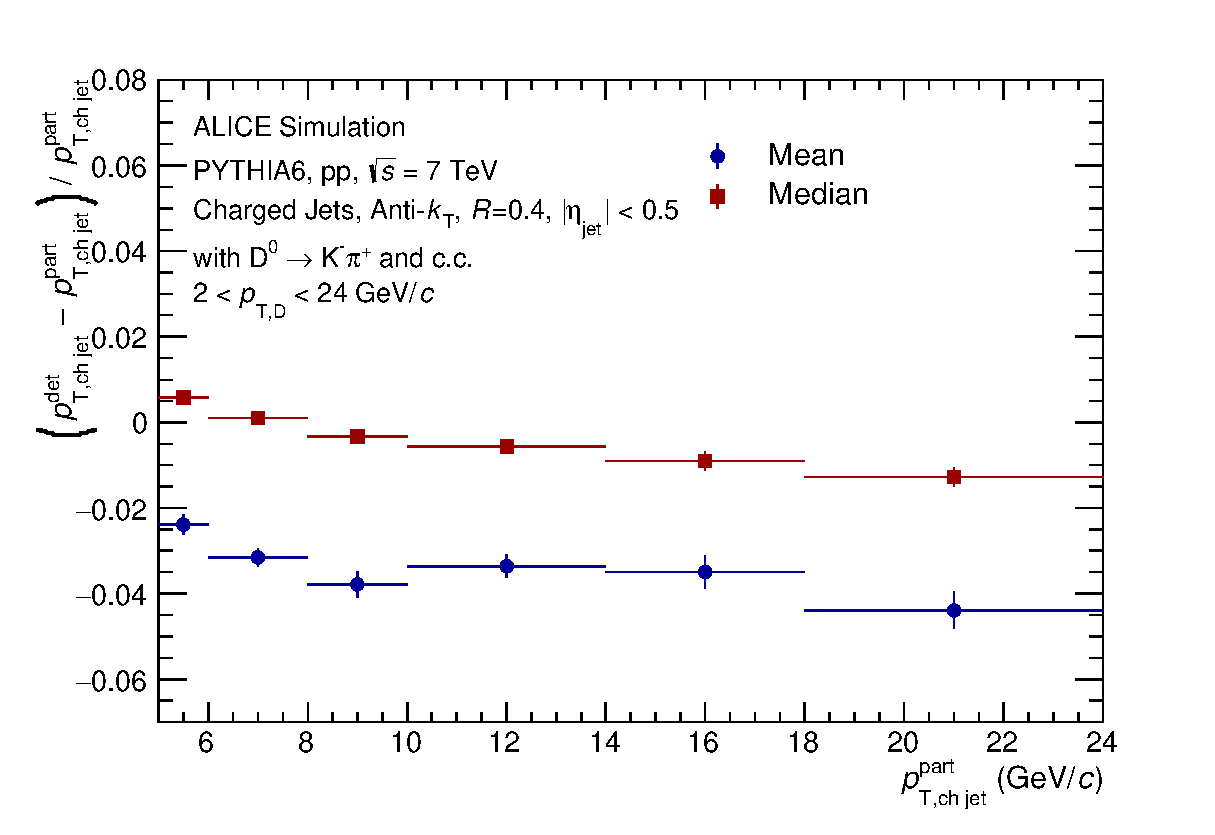
\includegraphics[width=1.0\linewidth]{img/HQ16_Simulation_EnergyScaleShift}
  \caption{Energy scale shift}
  \label{fig:HQ16_Simulation_EnergyScaleShift}
\end{subfigure}
\begin{subfigure}{0.49\textwidth}
  \centering
  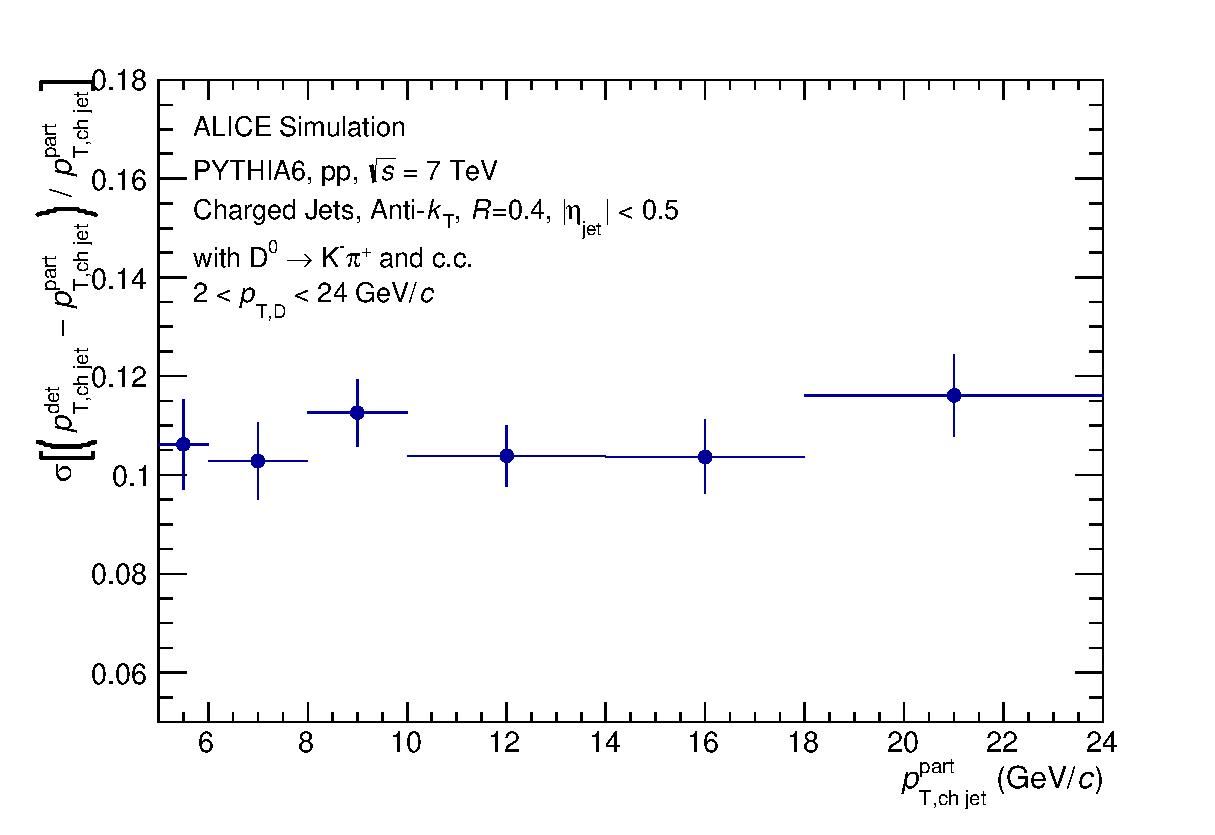
\includegraphics[width=1.0\linewidth]{img/HQ16_Simulation_Resolution}
  \caption{Resolution}
  \label{fig:HQ16_Simulation_Resolution}
\end{subfigure}
\caption{The variable (\ptchjetdet $-$ \ptchjetgen) / \ptchjetgen\ is used to estimate the corrections that need to be applied for the detector effects.}
\label{fig:DetectorResponse}
\end{figure}
%%%%
\subsection{Signal extraction}
%%%%
\begin{figure}[tbh]
\begin{center}
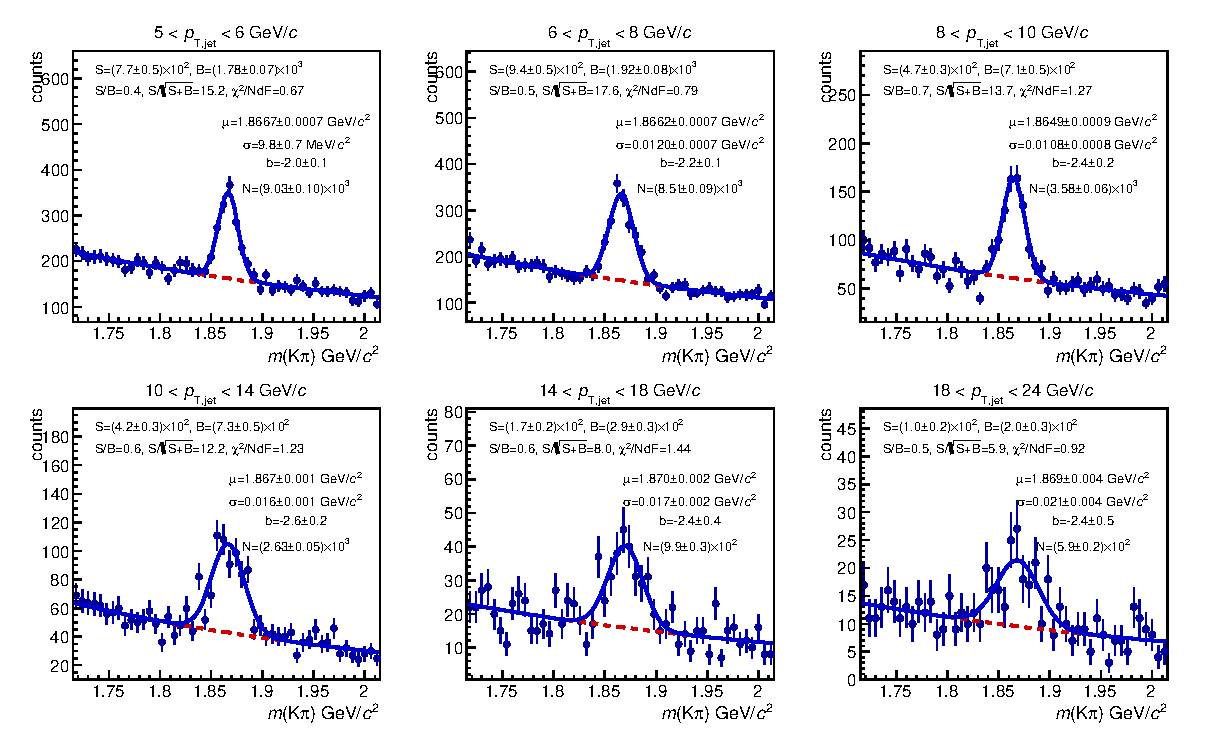
\includegraphics[width=0.8\textwidth]{img/D0_JetPtBins_PtD_20}
 \caption{Invariant mass distribution in bins of \ptchjetdet\ from simulation (LHC14j4b, LHC14j4c, LHC14j4d, LHC14j4e). The fit curves for background only (red) and signal plus background (blue) are superimposed.} 
 \label{fig:D0_JetPtBins_PtD_20}
\end{center}
\end{figure}

\begin{figure}[tbh]
\begin{center}
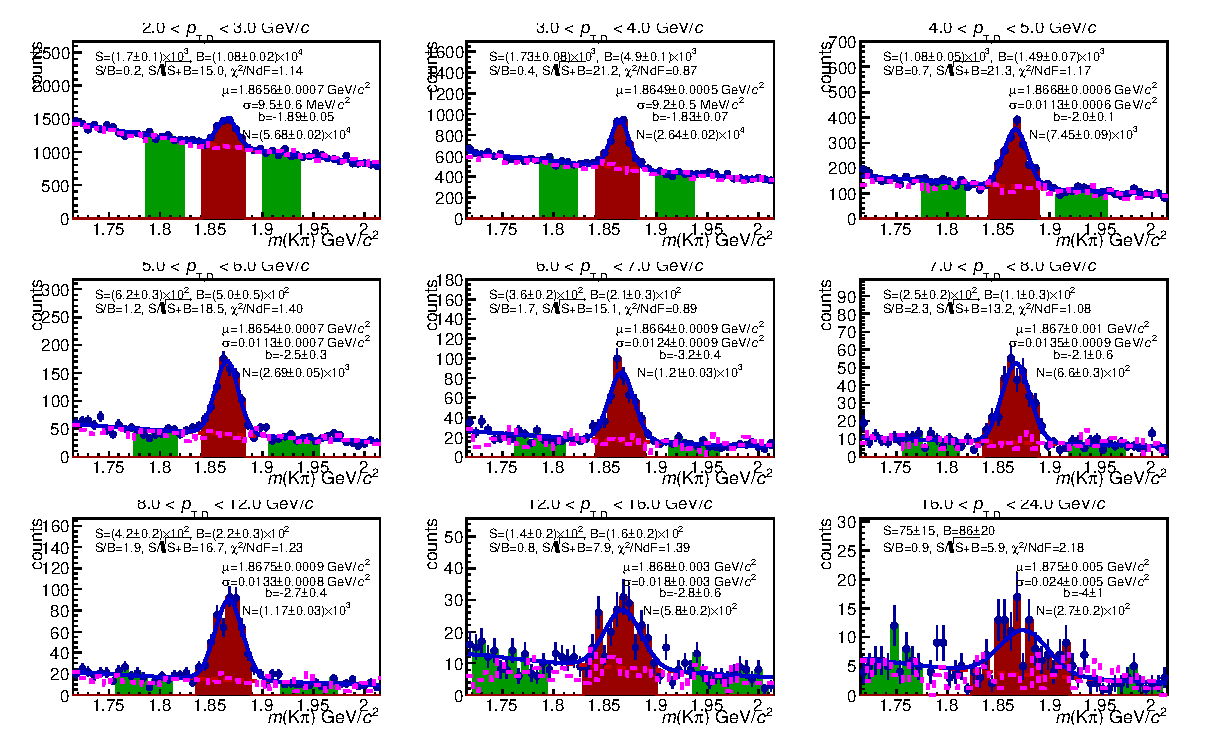
\includegraphics[width=0.8\textwidth]{img/D0_DPtBins_PtD_20}
 \caption{Invariant mass distribution for in bins of \ptd\ from simulation (LHC14j4b, LHC14j4c, LHC14j4d, LHC14j4e); the plot shows also the signal region, the S-B regions and the L-S invariant mass; the fit curves are show as well.} 
 \label{fig:D0_DPtBins_PtD_20}
\end{center}
\end{figure}
Three methods for the signal extraction have been implemented and tested in MC.
In the first method the \Dzero\ meson candidates are divided in bins of jet \pt. The invariant mass distributions
are fit using a Gaussian for the signal and an exponential function for the background, as shown in Fig.~\ref{fig:D0_JetPtBins_PtD_20}.
For the second and third methods the \Dzero\ candidates are divided in bins of \ptd. 
The invariant mass distributions in bins of \ptd\ are fit with the same function as above. The 
invariant mass distributions in bins of \ptd\ are shown in Fig.~\ref{fig:D0_DPtBins_PtD_20}. The
peak position and its width are estimated from the fit, as well as the amount of background 
in the peak region ($|M_{\mathrm{K\pi}}-M_{\mathrm{fit}}| < 2\sigma_{\mathrm{fit}}$).
Then for each \ptd\ bin the \ptchjet\ distribution of the \Dzero\ candidates is extracted.
For the side-band (S-B) method the background is estimated from the \ptchjet\ distribution 
of the \Dzero\ candidates in the side bands (\mbox{$4\sigma_{\mathrm{fit}} < |M_{\mathrm{K\pi}}-M_{\mathrm{fit}}| < 8\sigma_{\mathrm{fit}}$}),
as shown in Fig.~\ref{fig:D0_DPtBins_PtD_20}.
For the like-sign (L-S) method the background is estimated from the \ptchjet\ distribution of the like-sign pairs in the \Dzero\ peak region.
In both cases, the background \ptchjet\ distributions are normalized using the total background estimated from the invariant mass fit.
The normalized L-S invariant mass distributions are superimposed in Fig.~\ref{fig:D0_DPtBins_PtD_20} as well.
\begin{figure}[tbh]
\begin{center}
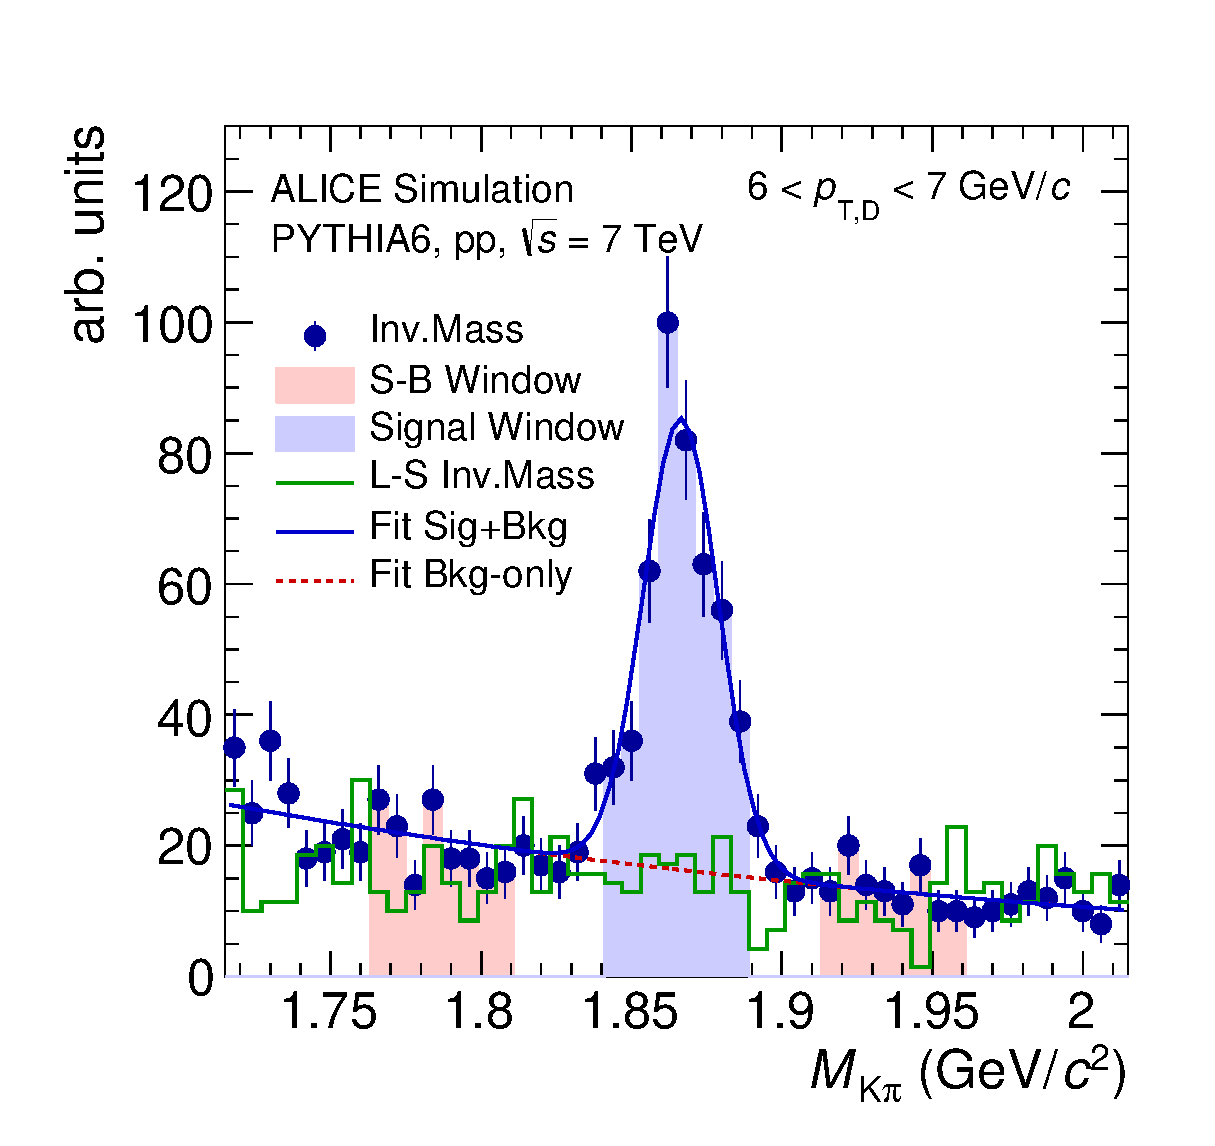
\includegraphics[width=0.8\textwidth]{img/HQ16_Simulation_InvMassSB}
 \caption{Invariant mass distribution for $6 < \ptd < 7$~\GeVc; the plot shows also the signal region, the S-B regions and the L-S invariant mass; the fit curves are shown as well.} 
 \label{fig:HQ16_Simulation_InvMassSB}
\end{center}
\end{figure}
Figure~\ref{fig:HQ16_Simulation_InvMassSB} shows the invariant mass distribution for $6 < \ptd < 7$~\GeVc. 

The signal extraction is validated by comparing the spectra obtained with the three methods outlined above with the MC truth. 
\begin{figure}[tbh]
\begin{center}
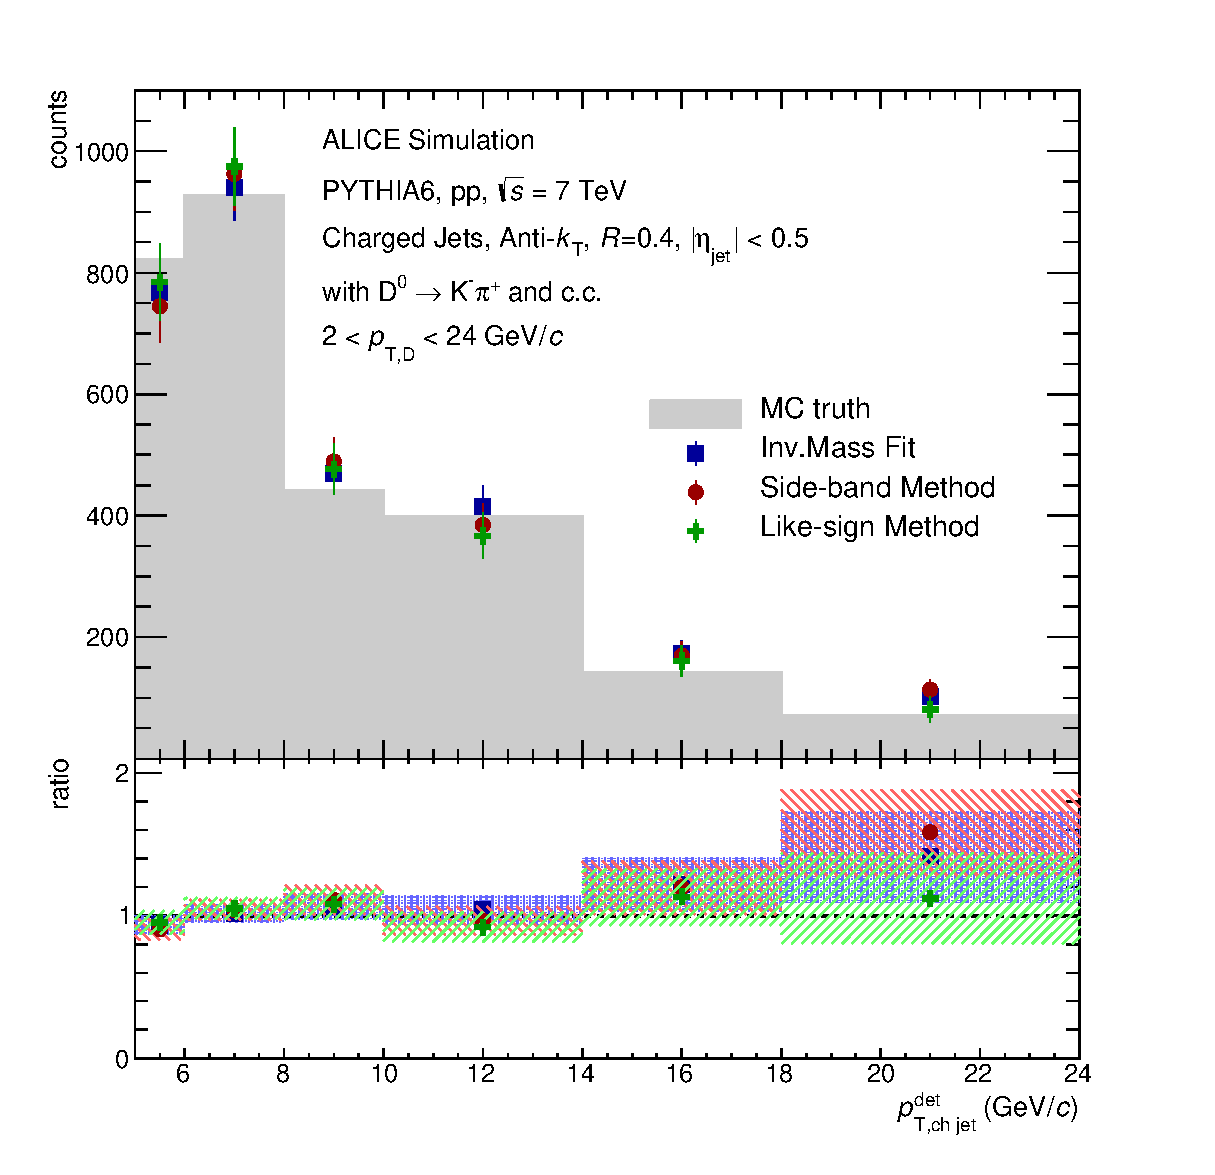
\includegraphics[width=0.8\textwidth]{img/HQ16_Simulation_MethodComparison}
 \caption{Comparison of the yields obtained using invariant mass fit, L-S and S-B methods.} 
 \label{fig:HQ16_Simulation_MethodComparison}
\end{center}
\end{figure}

\begin{figure}[tbh]
\begin{center}
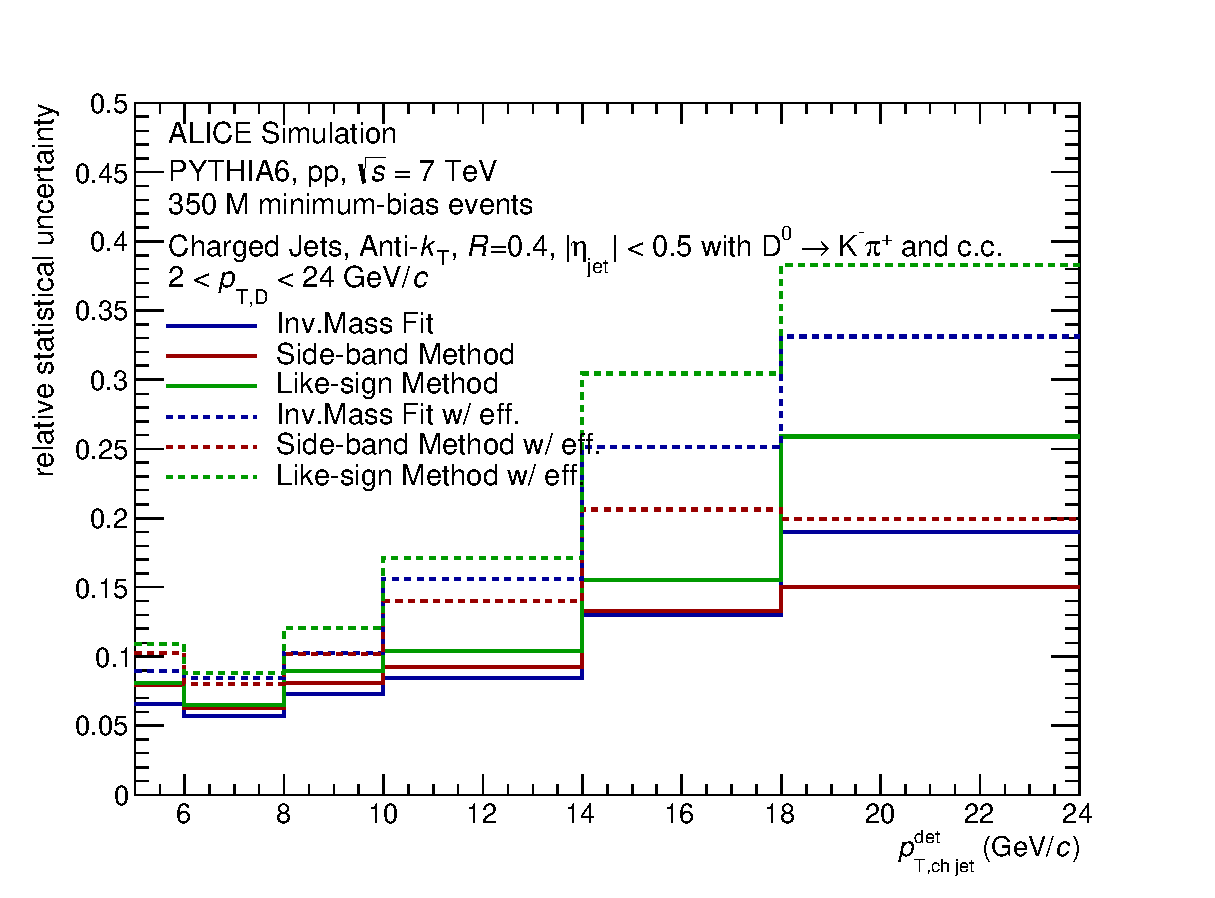
\includegraphics[width=0.8\textwidth]{img/HQ16_Simulation_UncertaintyComparison}
 \caption{Comparison of the statistical precisions obtained using invariant mass fit, L-S and S-B methods.} 
 \label{fig:HQ16_Simulation_UncertaintyComparison}
\end{center}
\end{figure}
The invariant mass fit, L-S and S-B methods all show good performances in recovering the signal, as shown in Fig.~\ref{fig:HQ16_Simulation_MethodComparison}.
The statistical uncertainties on the MC truth are ignored, as they are expected to be fully correlated with the signal extracted using any of the three methods.
The agreement between the signal extracted using the 3 methods and the MC truth has been tested using statistical analysis. The $\chi^2$ values
of the ratios data points compared to the expectation value of unity are 6.33, 11.25 and 3.05, respectively for the invariant mass fit, S-B and L-S methods.
These values quite close to the number of degrees of freedom ($=6$), except for the S-B method.
Calculating the $\chi^2$ on the single data points does not take into account correlated systematic shifts in a single direction. So another test that can be
done is to calculate the average of each ratio curve and compare it with unity. In this case the $\chi^2$ values are: 3.93, 5.94, 0.46, respectively for the invariant mass fit,
S-B and L-S methods (note that the number of degrees of freedom is now reduced to 5). These $\chi^2$ values correspond to $p$-values: 0.56, 0.31 and 0.994 (null hypothesis is
that there is no systematic shift).
This means that the probability that the data points are all systematically shifted in one direction (upward or downward) is 44\%, 69\% and 0.6\%, respectively.
In summary the possibility that there is a systematic shift cannot be excluded but is also not particularly significant. Comparing the signal extracted using the invariant mass fit
as a function of \ptd\, shown in Fig.~\ref{fig:YieldPtD}, one observes a upward fluctuation for the last bin ($16 < $~\ptd~$<24$~\GeVc). These yields are obtained from the invariant mass fits
shown in Fig.~\ref{fig:D0_DPtBins_PtD_20}. This could be the cause of the upward fluctuation observed in the last \ptchjet\ bin
in Fig.~\ref{fig:HQ16_Simulation_MethodComparison} for both the invariant mass fit and the S-B methods.
\begin{figure}[tbh]
\centering
\begin{subfigure}{0.49\textwidth}
  \centering
  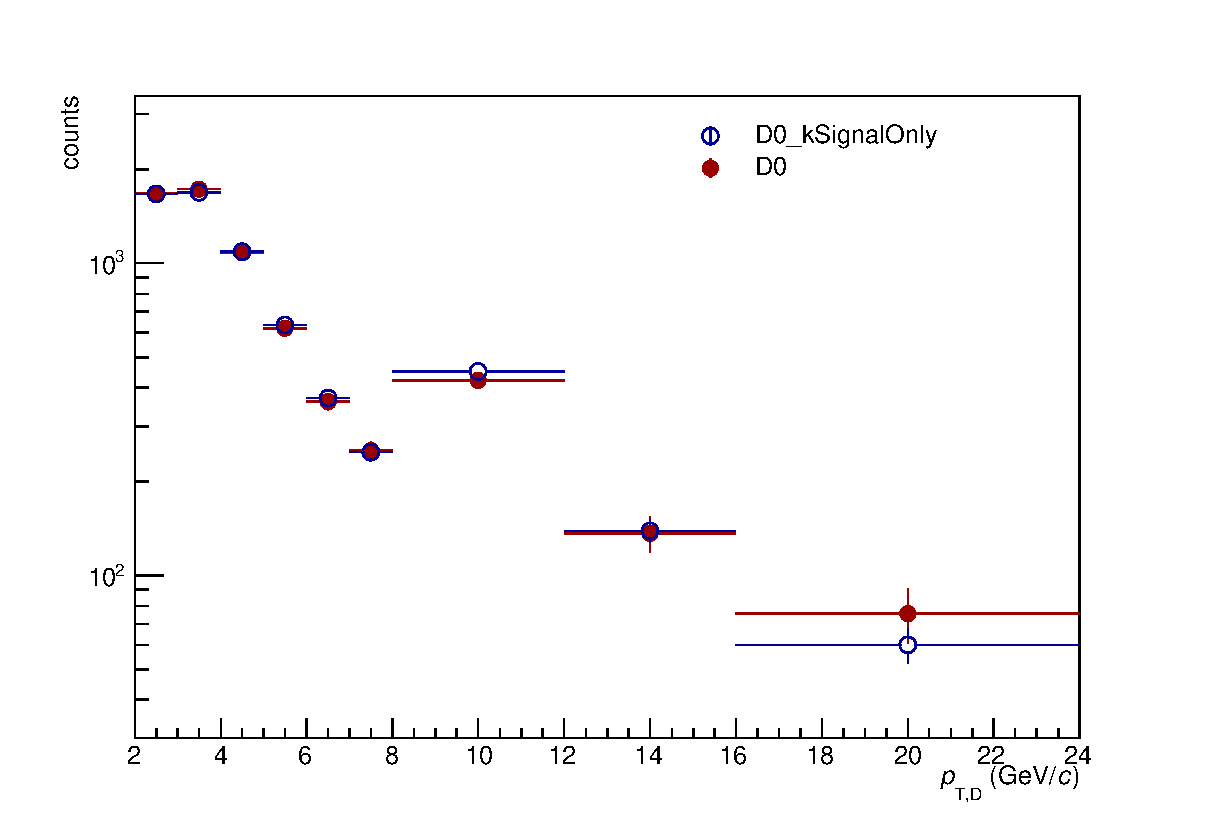
\includegraphics[width=1.0\linewidth]{img/D_Pt_Spectrum_SpectraComparison}
  \caption{Yields.}
\end{subfigure}
\begin{subfigure}{0.49\textwidth}
  \centering
  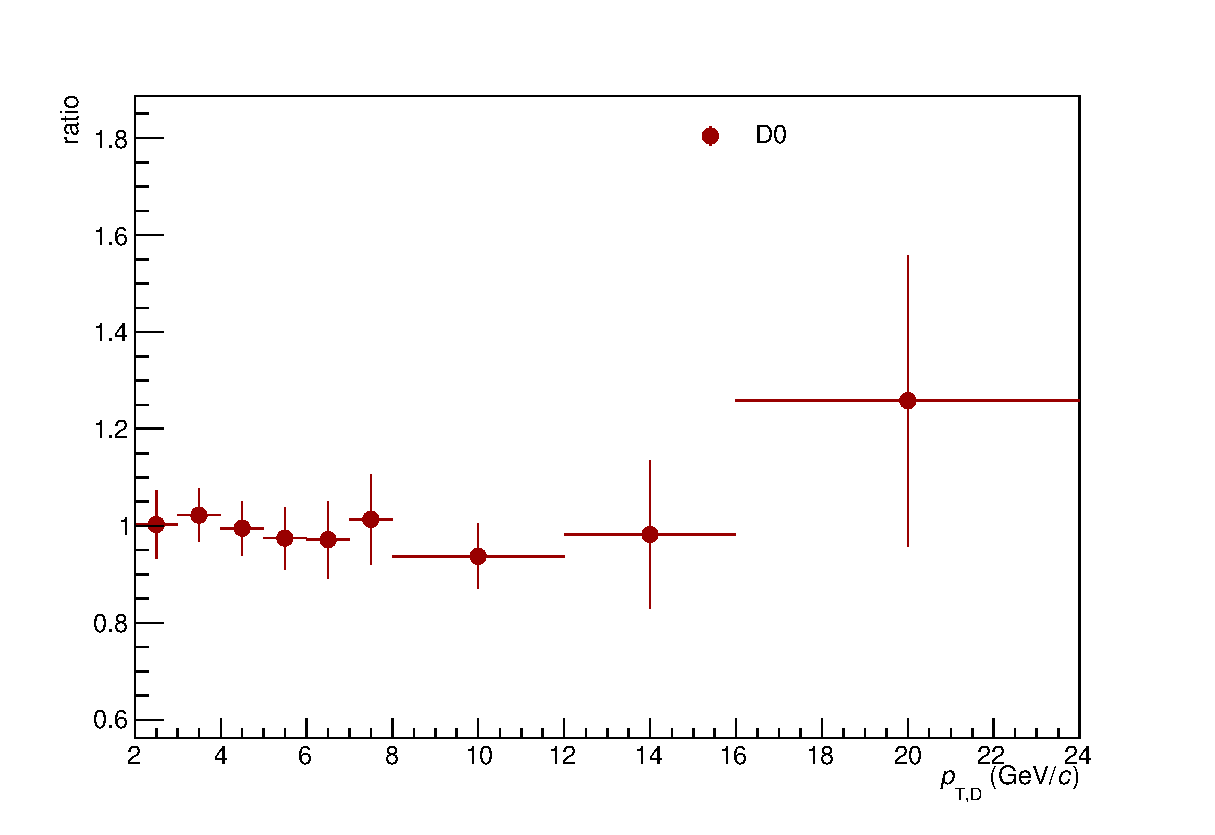
\includegraphics[width=1.0\linewidth]{img/D_Pt_Spectrum_SpectraComparison_Ratio}
  \caption{Ratio}
\end{subfigure}
\caption{Yield of D-tagged jets in bins of \ptd\ compared with MC truth.}
\label{fig:YieldPtD}
\end{figure}


For comparison, the difference (in counts) between the signal extracted using one of the 3 methods outlined above and the signal in the MC truth is shown in Fig.~\ref{fig:HQ16_Simulation_MethodComparison_Diff}.
\begin{figure}[tbh]
\begin{center}
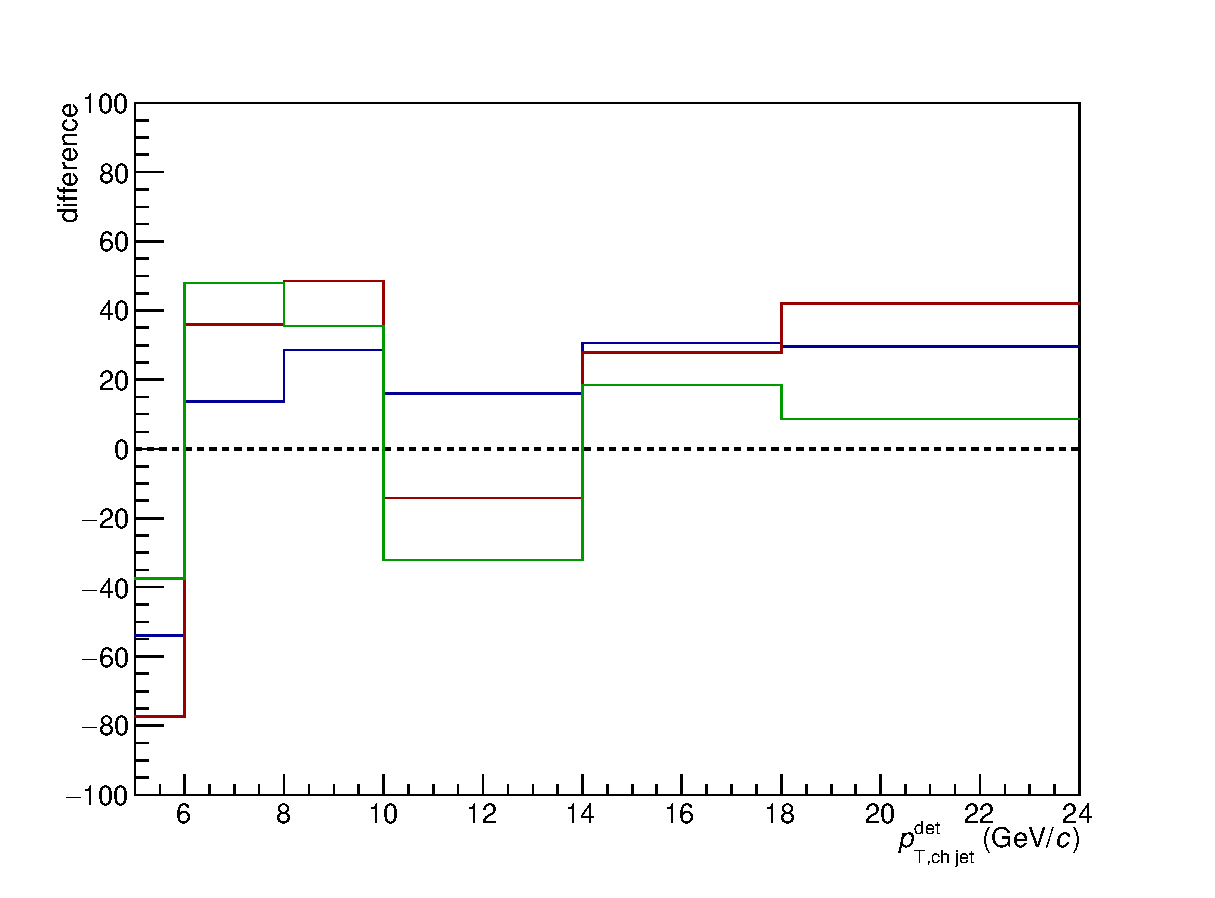
\includegraphics[width=0.8\textwidth]{img/HQ16_Simulation_MethodComparison_Diff}
 \caption{Difference between signal exctracted using the invariant mass fit (blue), the S-B (red) and the L-S (green) methods and the signal from the MC truth as a function of \ptchjetgen.} 
 \label{fig:HQ16_Simulation_MethodComparison_Diff}
\end{center}
\end{figure}

In Fig.~\ref{fig:HQ16_Simulation_UncertaintyComparison} the statistical precisions achieved by each method are compared. 
The statistical uncertainties are also shown for spectra corrected for the reconstruction efficiency. The efficiency correction alters the 
relative contribution of \Dzero\ mesons with different \pt\ in each \ptchjet\ bin. This is best illustrated in Figs.~\ref{fig:SigSpectra},~\ref{fig:SBSpectra},~\ref{fig:LSSpectra}, where the \ptchjetdet\ distributions
of D-tagged jet candidates are shown, respectively in the signal window, the S-B windows (both sides summed together) and the signal window of L-S pairs,
for different bins of \ptd. Low \ptd\ bins, that have few counts at high \ptchjetdet, get a larger efficiency weight compared to high \ptd\ bins, thus contributing more predominantly to both the signal and
its uncertainty in the high \ptchjetdet bins. On the other hand \ptd~$<$~\ptchjetdet\ (by construction), therefore the low \ptchjetdet\ bins suffer less from this effect because only low \ptd\ bins can contribute,
resulting in a less prominent remixing of the uncertainties.
\begin{figure}[tbh]
\centering
\begin{subfigure}{0.49\textwidth}
  \centering
  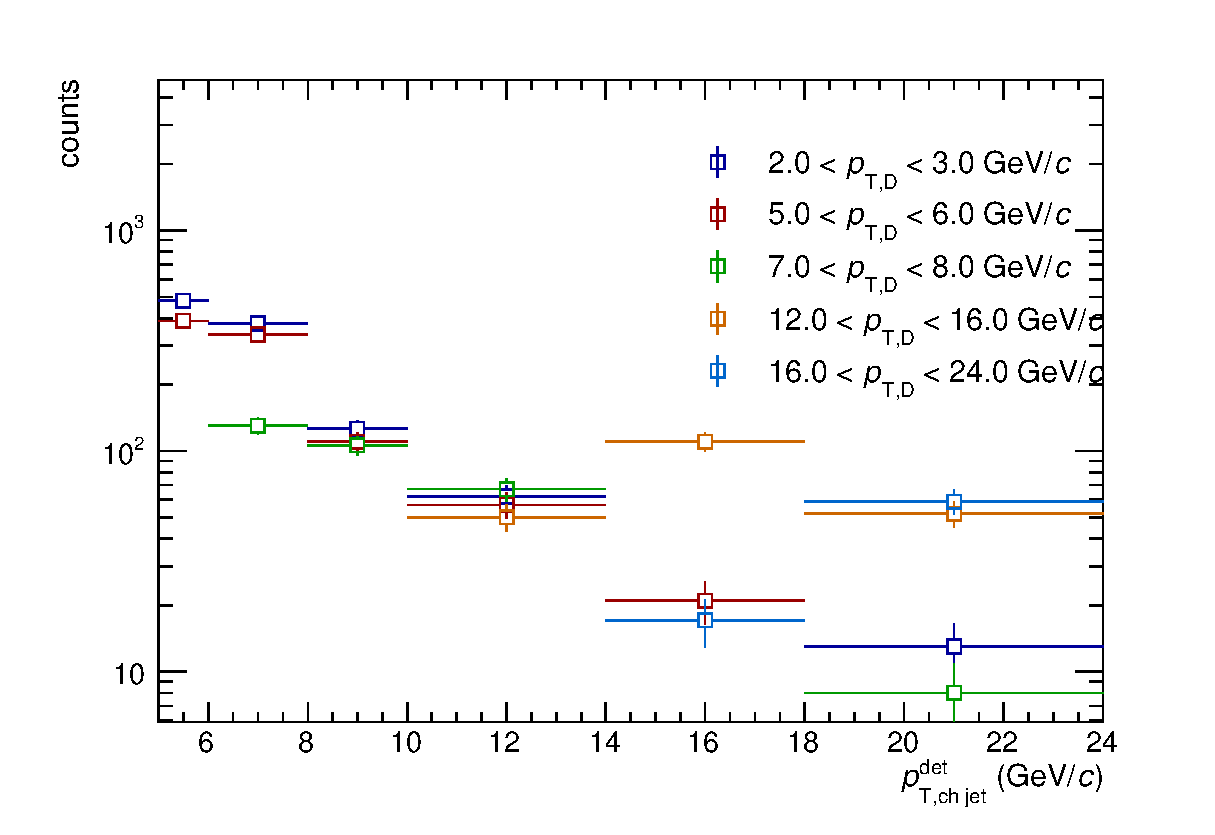
\includegraphics[width=1.0\linewidth]{img/HQ16_Simulation_SigSpectra}
  \caption{Without efficiency correction.}
\end{subfigure}
\begin{subfigure}{0.49\textwidth}
  \centering
  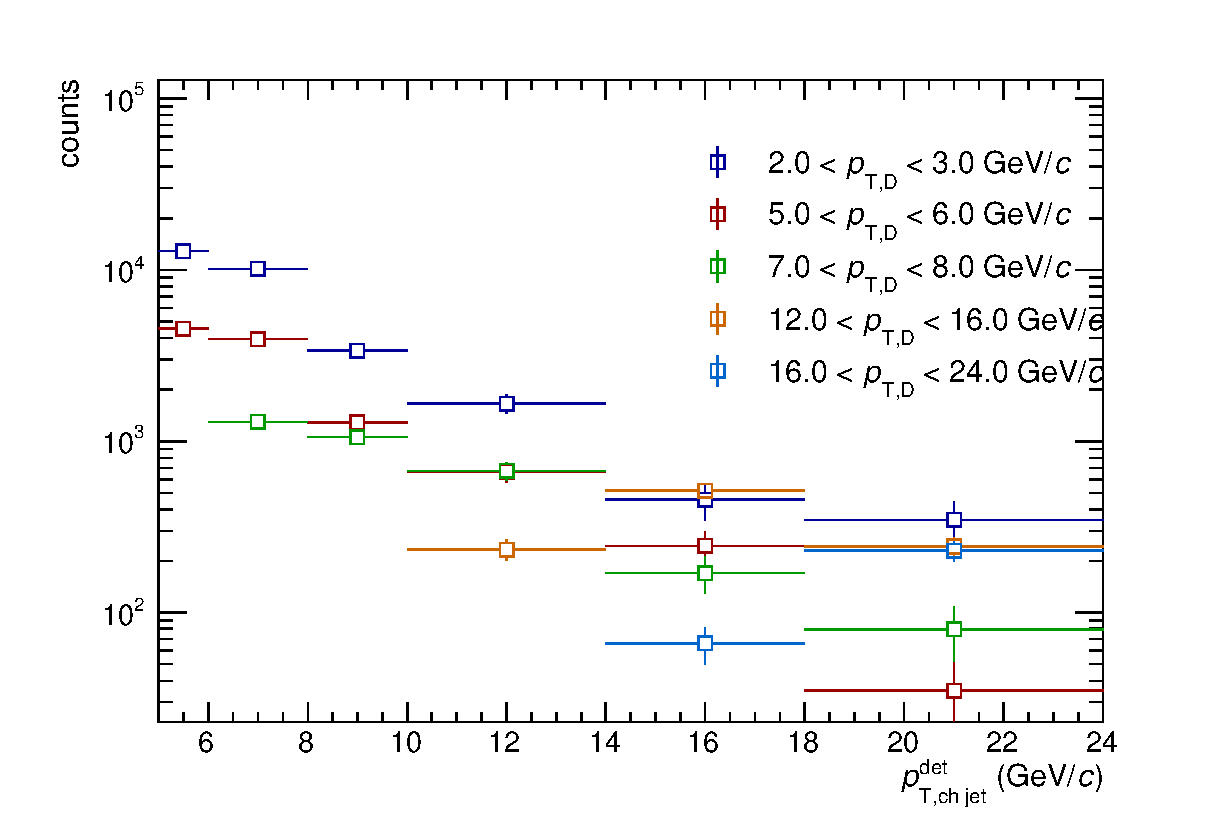
\includegraphics[width=1.0\linewidth]{img/HQ16_Simulation_SigSpectra_Eff}
  \caption{With efficiency correction}
\end{subfigure}
\caption{\ptchjetdet\ distributions of D-tagged jet candidates in the signal window for different bins of \ptd.}
\label{fig:SigSpectra}
\end{figure}

\begin{figure}[tbh]
\centering
\begin{subfigure}{0.49\textwidth}
  \centering
  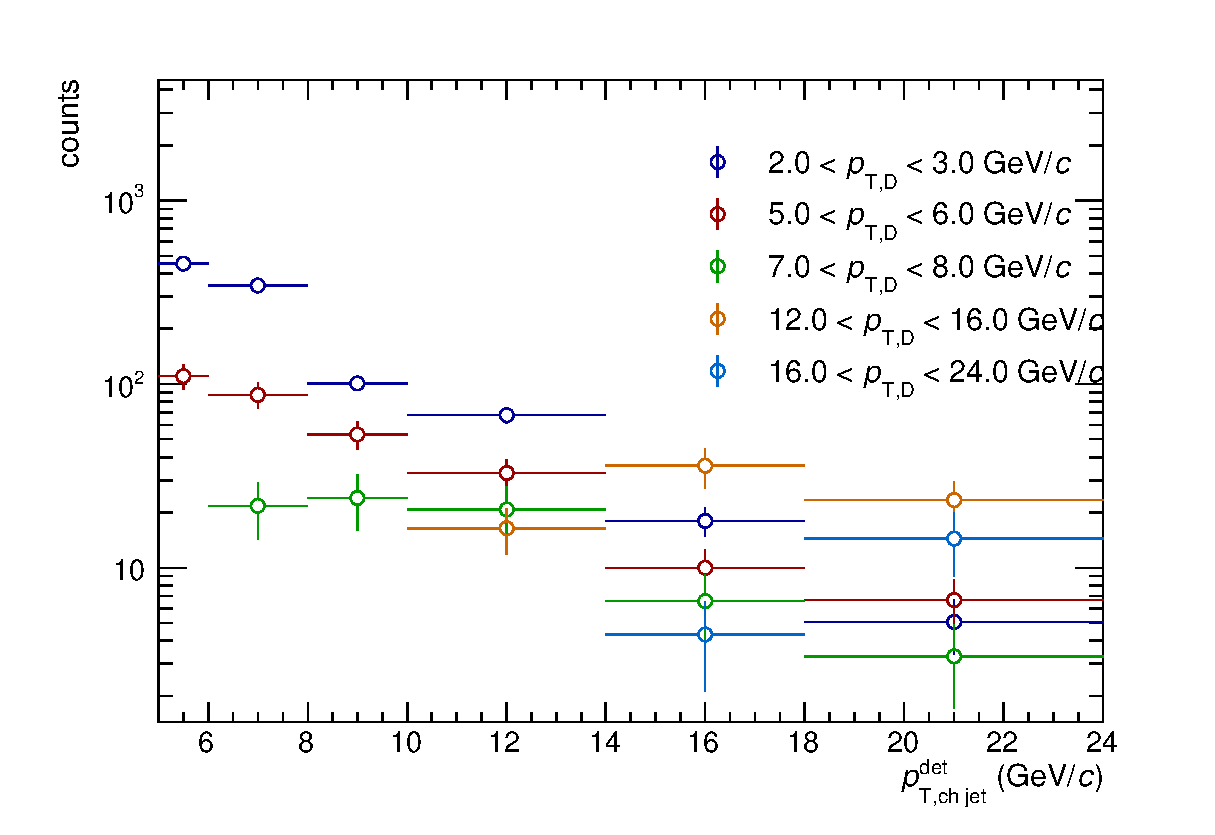
\includegraphics[width=1.0\linewidth]{img/HQ16_Simulation_SBSpectra}
  \caption{Without efficiency correction.}
\end{subfigure}
\begin{subfigure}{0.49\textwidth}
  \centering
  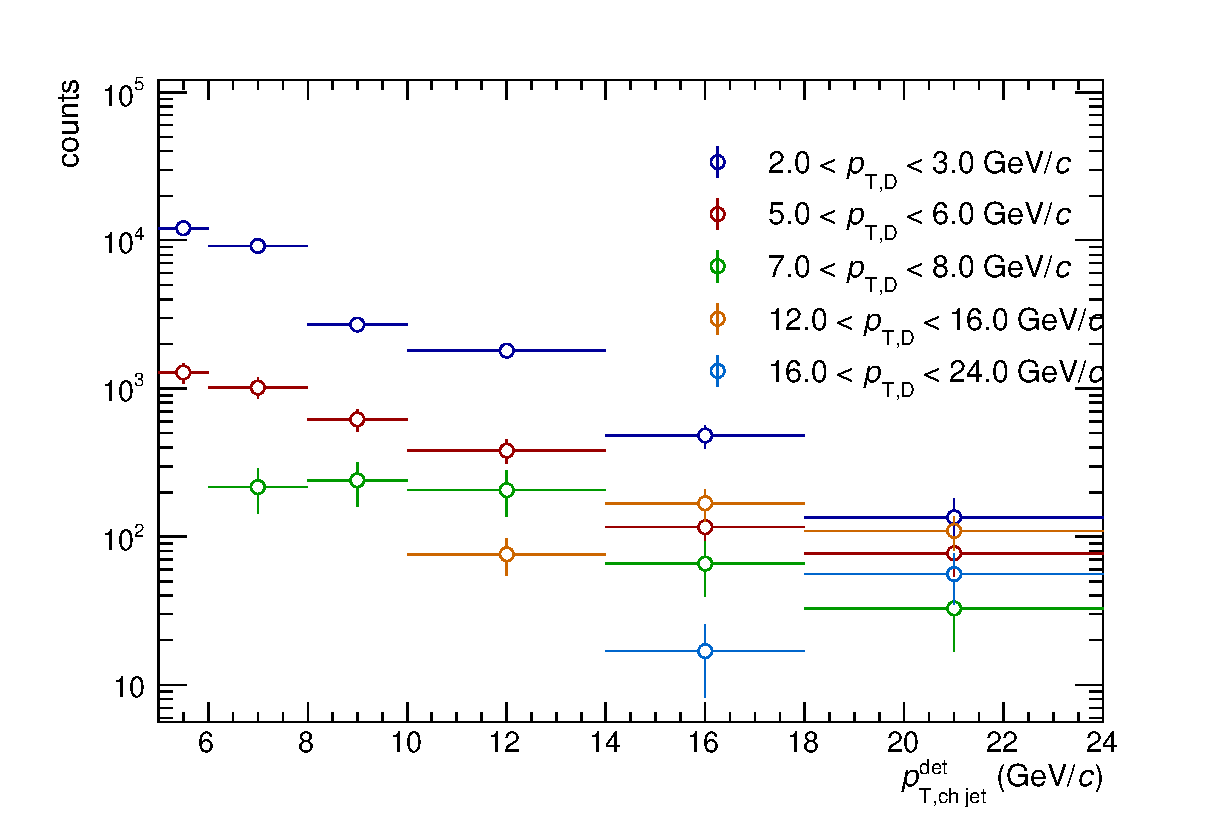
\includegraphics[width=1.0\linewidth]{img/HQ16_Simulation_SBSpectra_Eff}
  \caption{With efficiency correction}
\end{subfigure}
\caption{\ptchjetdet\ distributions of D-tagged jet candidates in the S-B window for different bins of \ptd.}
\label{fig:SBSpectra}
\end{figure}

\begin{figure}[tbh]
\centering
\begin{subfigure}{0.49\textwidth}
  \centering
  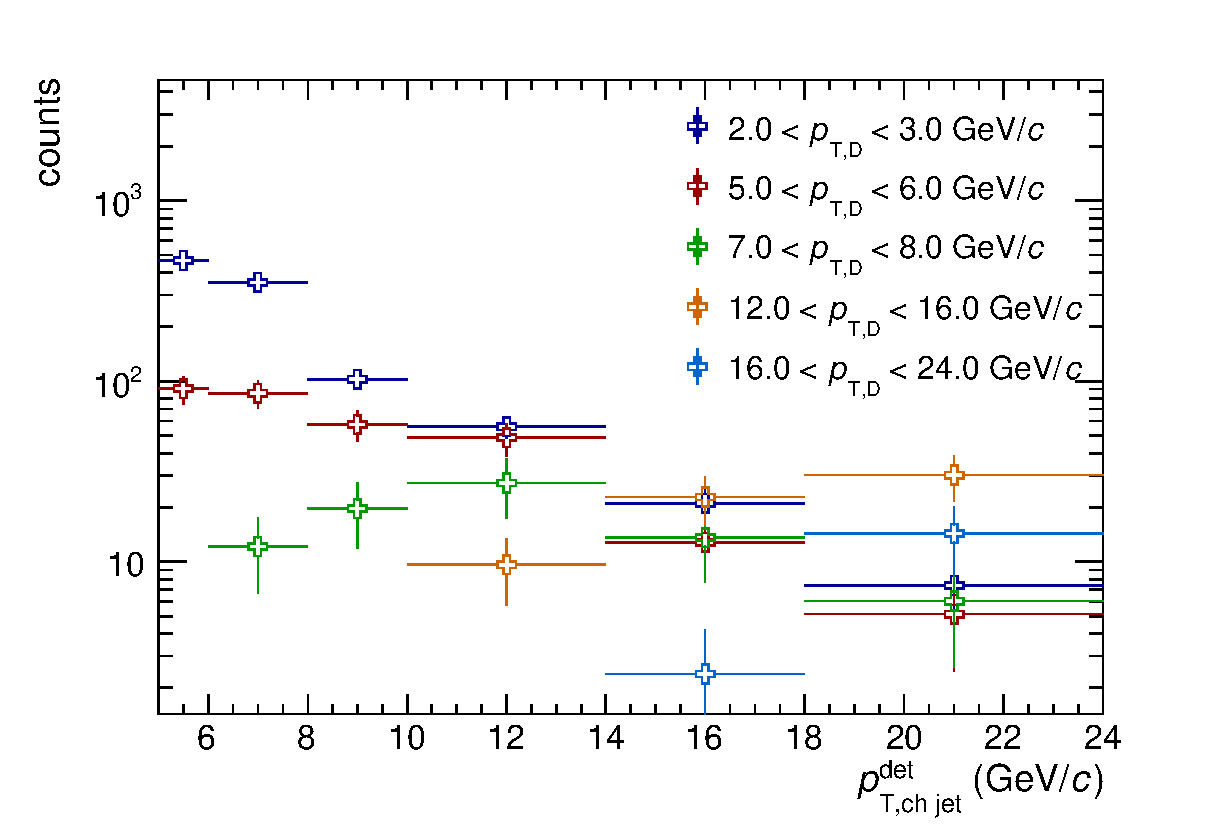
\includegraphics[width=1.0\linewidth]{img/HQ16_Simulation_LSSpectra}
  \caption{Without efficiency correction.}
\end{subfigure}
\begin{subfigure}{0.49\textwidth}
  \centering
  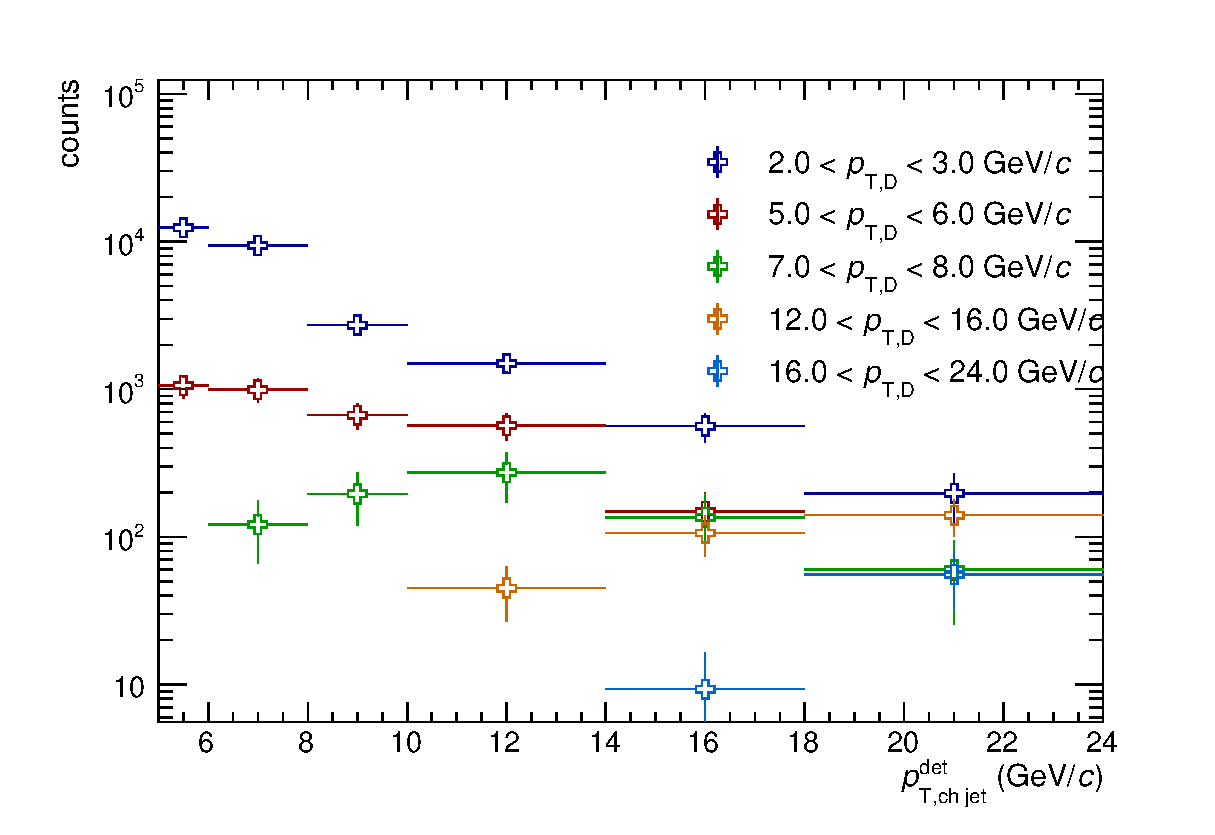
\includegraphics[width=1.0\linewidth]{img/HQ16_Simulation_LSSpectra_Eff}
  \caption{With efficiency correction}
\end{subfigure}
\caption{\ptchjetdet\ distributions of D-tagged jet candidates in the signal window for L-S pairs for different bins of \ptd.}
\label{fig:LSSpectra}
\end{figure}
%%%%%%%%%%%%
%%%%%%%%%%%%
\section{Work In Progress figure}
Figure~\ref{fig:HQ16_WorkInProgress_StatisticalUncertainty} is a work-in-progress plot that shows the statistical uncertainty 
of the D-tagged jets in all the available data for \pp\ collisions at \s~$=7$~TeV collected in 2010.
This corresponds to $316.41$ M minimum bias events. The signal is extracted via an invariant mass fit 
in jet \pt\ bins, as shown in Fig.~\ref{fig:D0_JetPtBins_PtD_20_Data}. 
Comparing Fig.~\ref{fig:D0_JetPtBins_PtD_20_Data} with Fig.~\ref{fig:HQ16_Simulation_UncertaintyComparison} one can
deduce some expectations about the statistical precisions of the other methods and/or after applying the efficiency correction.
However these expectations should only be considered of a qualitative nature, e.g.\ ``a significant loss of statistical precision
is expected after applying the efficiency correction'', or ``the L-S method is expected to have larger statistical uncertainty compared
to the invariant mass fit method''. The precise numbers depend on many aspects that may not be modeled correctly
in the MC generators, such as fragmentation and signal-over-background ratio.

These results come from the LEGO train Jets\_EMC\_pp run numbers: 764 (LHC10b),
765 (LHC10c), 766 (LHC10d), 767 (LHC10e). The AOD production pass4 has been used.
\begin{figure}[tbh]
\begin{center}
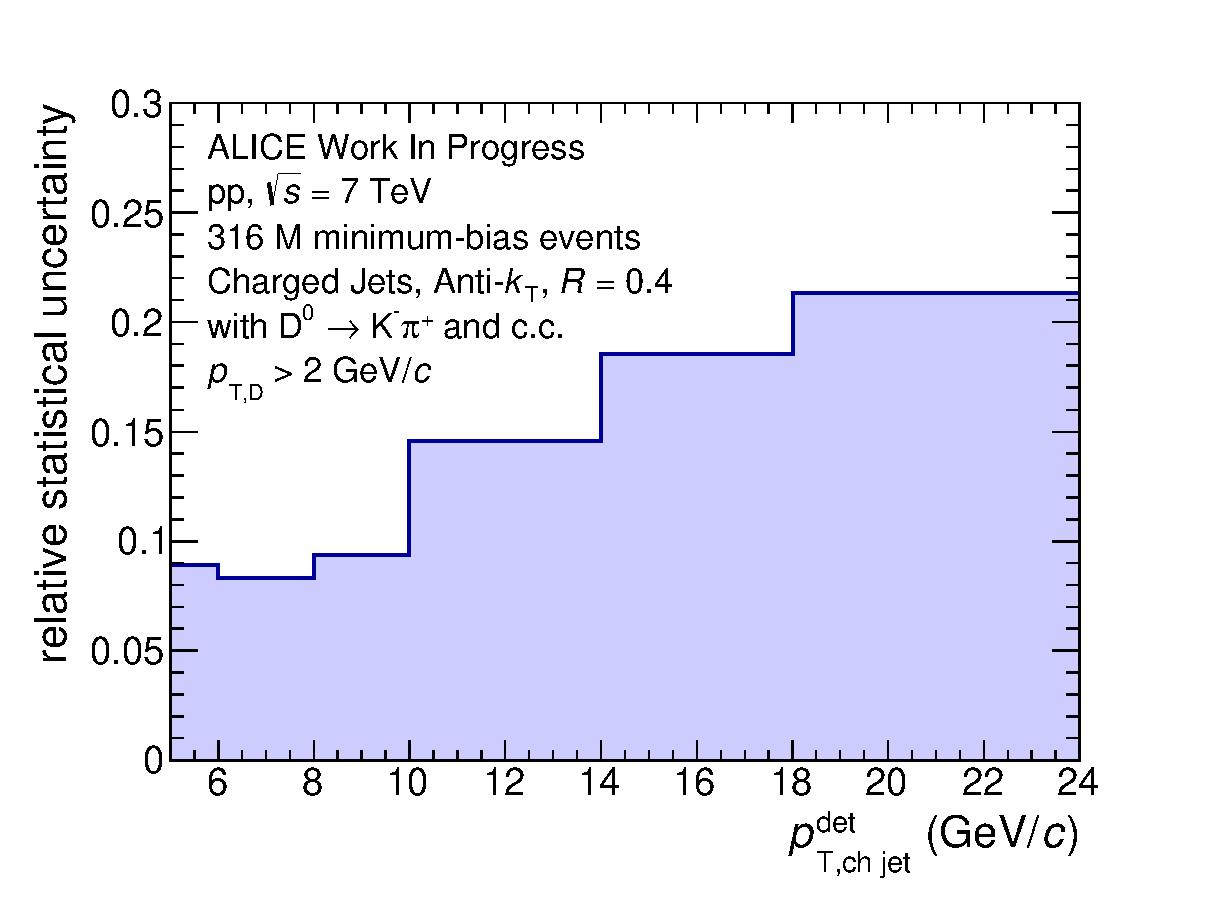
\includegraphics[width=0.8\textwidth]{img/HQ16_WorkInProgress_StatisticalUncertainty}
 \caption{Relative statistical uncertainty for D-tagged jets in 2010 pp data.} 
 \label{fig:HQ16_WorkInProgress_StatisticalUncertainty}
\end{center}
\end{figure}

\begin{figure}[tbh]
\begin{center}
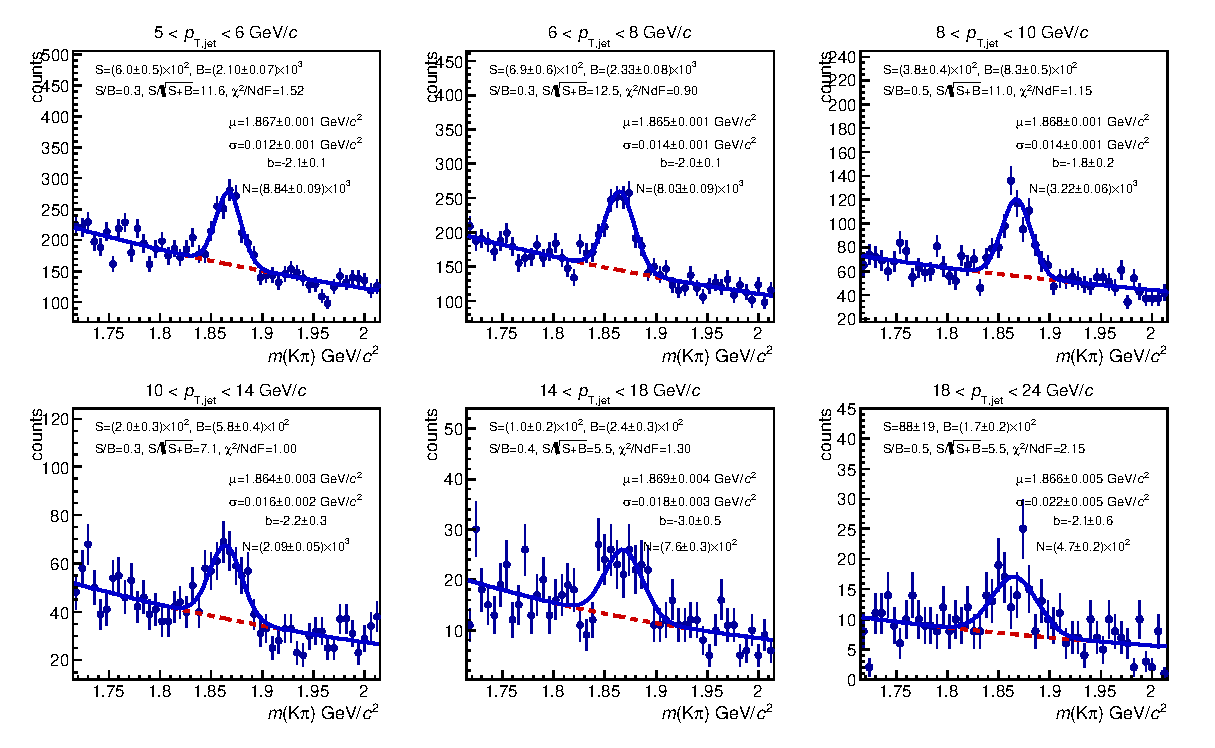
\includegraphics[width=0.8\textwidth]{img/D0_JetPtBins_PtD_20_Data}
 \caption{Invariant mass distribution in bins of \ptchjetdet\ from data (LHC10b, LHC10c, LHC10d, LHC10e). The fit curves for background only (red) and signal plus background (blue) are superimposed.} 
 \label{fig:D0_JetPtBins_PtD_20_Data}
\end{center}
\end{figure}
%%%%%%%%%%%%